% This LaTeX document needs to be compiled with XeLaTeX.
\documentclass[10pt]{article}
\usepackage[utf8]{inputenc}
\usepackage{amsmath}
\usepackage{amsfonts}
\usepackage{amssymb}
\usepackage[version=4]{mhchem}
\usepackage{stmaryrd}
\usepackage{graphicx}
\usepackage[export]{adjustbox}
\graphicspath{ {./images/} }
\usepackage{hyperref}
\hypersetup{colorlinks=true, linkcolor=blue, filecolor=magenta, urlcolor=cyan,}
\urlstyle{same}
\usepackage{multirow}
\usepackage[fallback]{xeCJK}
\usepackage{polyglossia}
\usepackage{fontspec}
\setCJKmainfont{Noto Serif CJK TC}

\setmainlanguage{polish}
\setmainfont{CMU Serif}

\title{PRÓBNY EGZAMIN MATURALNY Z MATEMATYKI }

\author{Czas pracy 170 minut}
\date{}


%New command to display footnote whose markers will always be hidden
\let\svthefootnote\thefootnote
\newcommand\blfootnotetext[1]{%
  \let\thefootnote\relax\footnote{#1}%
  \addtocounter{footnote}{-1}%
  \let\thefootnote\svthefootnote%
}

%Overriding the \footnotetext command to hide the marker if its value is `0`
\let\svfootnotetext\footnotetext
\renewcommand\footnotetext[2][?]{%
  \if\relax#1\relax%
    \ifnum\value{footnote}=0\blfootnotetext{#2}\else\svfootnotetext{#2}\fi%
  \else%
    \if?#1\ifnum\value{footnote}=0\blfootnotetext{#2}\else\svfootnotetext{#2}\fi%
    \else\svfootnotetext[#1]{#2}\fi%
  \fi
}

\begin{document}
\maketitle
\section*{POZIOM PODSTAWOWY}


\section*{Instrukcja dla piszącego}
\begin{enumerate}
  \item Sprawdź, czy arkusz zawiera 16 stron.
  \item W zadaniach od 1. do 20. są podane 4 odpowiedzi: \(\mathrm{A}, \mathrm{B}, \mathrm{C}, \mathrm{D}\), z których tylko jedna jest prawdziwa. Wybierz tylko iedna odpowiedź i zaznacz ją na karcie odpowiedzi.
  \item Zaznaczając odpowiedzi w części karty przeznaczonej dla zdającego, zamaluj \(\square\) pola do tego przeznaczone. Błędne zaznaczenie otocz kółkiem i zaznacz właściwe.
  \item Rozwiązania zadań od 21. do 30. zapisz starannie i czytelnie w wyznaczonych miejscach. Przedstaw swój tok rozumowania prowadzący do ostatecznego wyniku.
  \item Pisz czytelnie. Używaj długopisu/pióra tylko z czarnym tuszem/atramentem.
  \item Nie używaj korektora. Błędne zapisy przekreśl.
  \item Pamiętaj, że zapisy w brudnopisie nie podlegają ocenie.
  \item Obok numeru każdego zadania jest podana maksymalna liczba punktów możliwych do uzyskania.
  \item Możesz korzystać z zestawu wzorów matematycznych, cyrkla i linijki oraz kalkulatora.
  \item Wypełnij tę część karty odpowiedzi, którą koduje zdający. Nie wpisuj żadnych znaków w częşci przeznaczonej dla egzaminatora.
\end{enumerate}

Życzymy powodzenia!

Za rozwiązanie wszystkich zadań można otrzymać łącznie do\\
50 punktów

Wypelnia zdajacy przed\\
rozpoczęciem pracy\\

\includegraphics[max width=\textwidth, center]{2024_11_21_6438f6dbc3784fe6d1deg-01}

PESEL ZDAJĄCEGO

Odpowiedzi z tej próbnej matury znajdziesz dziś o godzinie 14 na \href{http://www.echodnia.eu/edukacja}{www.echodnia.eu/edukacja} oraz w jutrzejszym wydaniu papierowym „Echa Dnia"

\section*{ZADANIA ZAMKNIĘTE}
\section*{W zadaniach od 1. do 20. wybierz jedna poprawna odpowiedź.}
\section*{Zadanie 1. (1 pkt)}
Liczba \(32: \frac{1}{32} \cdot\left(-2^{10}\right)\) jest równa\\
A. \(-2^{10}\)\\
B. \(-2^{20}\)\\
C. \(2^{20}\)\\
D. \(2^{10}\)

\section*{Zadanie 2. (1 pkt)}
Pole kwadratu o boku długości \(4+3 \sqrt{2}\) jest równe\\
A. 34\\
B. 1008\\
C. \(14+9 \sqrt{2}\)\\
D. \(34+24 \sqrt{2}\)

\section*{Zadanie 3. (1 pkt)}
Liczba \(|1-\sqrt{3}|-|-5|\) jest równa\\
A. \(6+\sqrt{3}\)\\
B. \(6-\sqrt{3}\)\\
C. \(-6-\sqrt{3}\)\\
D. \(-6+\sqrt{3}\)

\section*{Zadanie 4. (1 pkt)}
Cena komputera wraz z 23\% podatkiem VAT jest równa 5166 zł. Cena tego komputera bez podatku VAT jest równa\\
A. 3978 zl\\
B. 4200 zl\\
C. 5143 zf\\
D. 6354 zl

Zadanie 5. (1 pkt)\\
Liczba \(2 \log _{3} 12-\log _{3} 16\) jest równa\\
A. 2\\
B. -8\\
C. 9\\
D. \(\frac{3}{2}\)

\section*{Zadanie 6. (1 pkt)}
Zbiorem rozwiązań nierówności \((x-3)(x+4) \leq 0\) jest\\
A. \((-\infty,-3\rangle \cup\langle 4,+\infty)\)\\
B. \(\langle-3,4\rangle\)\\
C. \(\langle-4,3\rangle\)\\
D. \((-\infty,-4\rangle \cup\langle 3,+\infty)\)

\section*{Zadanie 7. (1 pkt)}
Liczby \(x-2,4,2\) są, w podanej kolejności, odpowiednio pierwszym, drugim i trzecim wyrazem ciągu geometrycznego. Wówczas\\
A. \(x=10\)\\
B. \(x=8\)\\
C. \(x=4\)\\
D. \(x=2\)

\section*{Zadanie 8. (1 pkt)}
W ciągu arytmetycznym \(\left(a_{n}\right)\) dane są \(a_{1}=3\) i \(a_{2}=7\). Wtedy\\
A. \(a_{6}=23\)\\
B. \(a_{6}=27\)\\
C. \(a_{6}=\frac{16807}{81}\)\\
D. \(a_{6}=60\)

\section*{BRUDNOPIS}
Zadanie 9. (1 pkt)\\
Proste o równaniach \(-2 x+y+5=0\) i \(y=(3-m) x+4\) są równoległe. Wynika stąd, że\\
A. \(m=-\frac{2}{3}\)\\
B. \(m=1\)\\
C. \(m=\frac{3}{2}\)\\
D. \(m=5\)

\section*{Zadanie 10. (1 pkt)}
Długości dwóch boków trójkąta prostokątnego i kąt ostry \(\alpha\) tego trójkąta są zaznaczone na rysunku. Wówczas\\
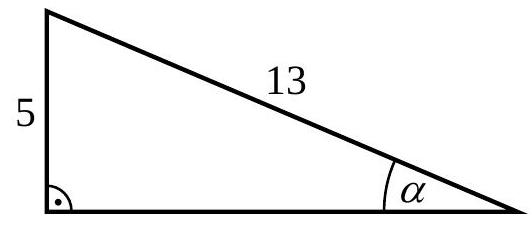
\includegraphics[max width=\textwidth, center]{2024_11_21_6438f6dbc3784fe6d1deg-04(1)}\\
A. \(\sin \alpha=\frac{5}{13}\)\\
B. \(\cos \alpha=\frac{5}{13}\)\\
C. \(\operatorname{tg} \alpha=\frac{5}{13}\)\\
D. \(\operatorname{tg} \alpha=\frac{13}{5}\)

\section*{Zadanie 11. (1 pkt)}
Równanie okręgu o środku \(S=(-4,1)\) i promieniu \(r=4\) ma postać\\
A. \((x-4)^{2}+(y+1)^{2}=4\)\\
B. \((x+4)^{2}+(y-1)^{2}=4\)\\
C. \((x-4)^{2}+(y+1)^{2}=16\)\\
D. \((x+4)^{2}+(y-1)^{2}=16\)

\section*{Zadanie 12. (1 pkt)}
Równanie \(x^{5}-9 x^{3}=0\)\\
A. nie ma rozwiązań.\\
B. ma dokładnie jedno rozwiązanie \(x=3\).\\
C. ma dokładnie dwa rozwiązania: \(x=-3, x=3\).\\
D. ma dokładnie trzy rozwiązania: \(x=-3, x=0, x=3\).

\section*{Zadanie 13. (1 pkt)}
Proste \(A C\) i \(B D\) są równoległe. Długości odcinków \(E C, C D\) oraz \(A B\) podane są na rysunku. Długość odcinka EA jest równa\\
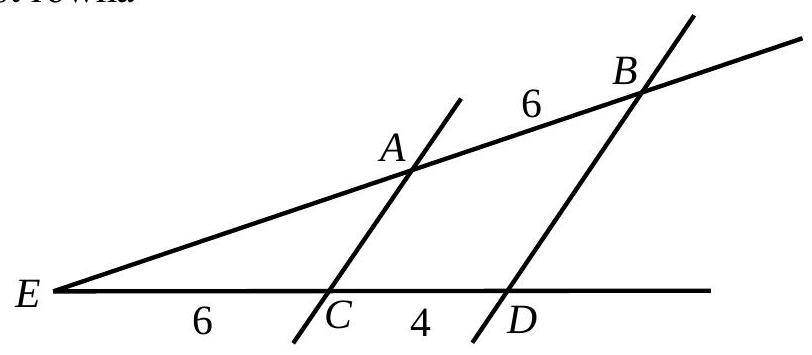
\includegraphics[max width=\textwidth, center]{2024_11_21_6438f6dbc3784fe6d1deg-04}\\
A. 4\\
B. 8\\
C. 9\\
D. 10

Zadanie 14. (1 pkt)\\
Zbiorem wartości funkcji kwadratowej \(f(x)=2 x^{2}+4 x-16\) jest\\
A. \((-4,2)\)\\
B. \((-16,+\infty)\)\\
C. \(\langle-16,+\infty)\)\\
D. \(\langle-18,+\infty)\)

\section*{BRUDNOPIS}
Zadanie 15. (1 pkt)\\
Dla każdego \(x \neq-2\) wyrażenie \(\frac{x-1}{2 x+4}: \frac{2}{x+2}\) jest równe\\
A. \(\frac{x^{2}-x}{2 x+4}\)\\
B. \(\frac{x+1}{3 x+6}\)\\
C. \(\frac{x-1}{4}\)\\
D. \(\frac{x-1}{(x+2)^{2}}\)

Zadanie 16. (1 pkt)\\
Kąt między cięciwą \(A B\) oraz styczną do okręgu poprowadzoną przez punkt \(A\) ma miarę \(\alpha=42^{\circ}\). Wówczas miara kąta wpisanego \(A C B\) (zobacz rysunek) jest równa\\
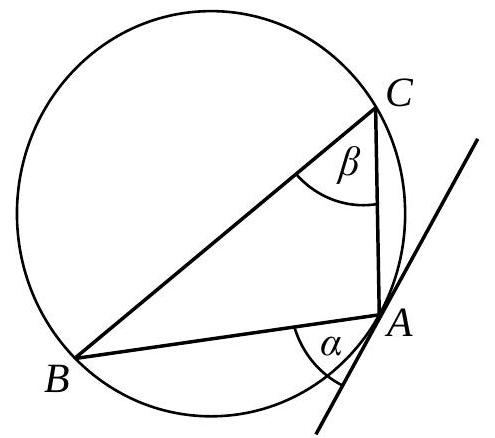
\includegraphics[max width=\textwidth, center]{2024_11_21_6438f6dbc3784fe6d1deg-06}\\
A. \(\beta=21^{\circ}\)\\
B. \(\beta=42^{\circ}\)\\
C. \(\beta=48^{\circ}\)\\
D. \(\beta=84^{\circ}\)

\section*{Zadanie 17.}
Wykres funkcji \(f(x)=2^{x}\) przesunięto wzdłuż osi Ox o 1 jednostkę w lewo otrzymując wykres funkcji\\
A. \(g(x)=2^{x}-1\)\\
B. \(g(x)=2^{x-1}\)\\
C. \(g(x)=2^{x}+1\)\\
D. \(g(x)=2^{x+1}\)

Zadanie 18. (1 pkt)\\
Czworo znajomych: Adam, Beata, Czarek i Dorota mają bilety na miejsca 11, 12, 13 i 14 w VIII rzędzie sali kinowej. Na ile sposobów mogą oni wszyscy zając te miejsca tak, żeby Adam siedział obok Beaty i Czarek obok Doroty?\\
A. 24\\
B. 8\\
C. 4\\
D. 2

Zadanie 19. (1 pkt)\\
Mediana danych przedstawionych w tabeli liczebności jest równa

\begin{center}
\begin{tabular}{|c|c|c|c|c|}
\hline
wartość & 0 & 1 & 2 & 3 \\
\hline
liczebność & 2 & 2 & 1 & 5 \\
\hline
\end{tabular}
\end{center}

A. \(\frac{3}{2}\)\\
B. 2\\
C. \(\frac{5}{2}\)\\
D. 3

Zadanie 20. (1 pkt)\\
O zdarzeniach \(A\) oraz \(B\) zawartych w \(\Omega\) wiadomo, że \(A \subset B, P(A)=\frac{1}{6}, P(B)=\frac{2}{3}\). Wtedy\\
A. \(\quad P(A \cup B)=\frac{5}{6}\)\\
B. \(\quad P(A \cup B)=\frac{1}{2}\)\\
C. \(P(A \cup B)=\frac{2}{3}\)\\
D. \(\quad P(A \cup B)=\frac{1}{6}\)

\section*{BRUDNOPIS}
Zadanie 21. (2 pkt)\\
Rozwiąż nierówność \((x+2) \cdot(2-x)-\frac{(x+2)^{2}}{2} \leq-\frac{3}{2} x^{2}\).

\begin{center}
\begin{tabular}{|c|c|c|c|c|c|c|c|c|c|c|c|c|c|c|c|c|c|c|c|c|c|c|c|c|c|c|c|c|c|}
\hline
 &  &  &  &  &  &  &  &  &  &  &  &  &  &  &  &  &  &  &  &  &  &  &  &  &  &  &  &  &  \\
\hline
 &  &  &  &  &  &  &  &  &  &  &  &  &  &  &  &  &  &  &  &  &  &  &  &  &  &  &  &  &  \\
\hline
 &  &  &  &  &  &  &  &  &  &  &  &  &  &  &  &  &  &  &  &  &  &  &  &  &  &  &  &  &  \\
\hline
 &  &  &  &  &  &  &  &  &  &  &  &  &  &  &  &  &  &  &  &  &  &  &  &  &  &  &  &  &  \\
\hline
 &  &  &  &  &  &  &  &  &  &  &  &  &  &  &  &  &  &  &  &  &  &  &  &  &  &  &  &  &  \\
\hline
 &  &  &  &  &  &  &  &  &  &  &  &  &  &  &  &  &  &  &  &  &  &  &  &  &  &  &  &  &  \\
\hline
 &  &  &  &  &  &  &  &  &  &  &  &  &  &  &  &  &  &  &  &  &  &  &  &  &  &  &  &  &  \\
\hline
 &  &  &  &  &  &  &  &  &  &  &  &  &  &  &  &  &  &  &  &  &  &  &  &  &  &  &  &  &  \\
\hline
 &  &  &  &  &  &  &  &  &  &  &  &  &  &  &  &  &  &  &  &  &  &  &  &  &  &  &  &  &  \\
\hline
 &  &  &  &  &  &  &  &  &  &  &  &  &  &  &  &  &  &  &  &  &  &  &  &  &  &  &  &  &  \\
\hline
 &  &  &  &  &  &  &  &  &  &  &  &  &  &  &  &  &  &  &  &  &  &  &  &  &  &  &  &  &  \\
\hline
 &  &  &  &  &  &  &  &  &  &  &  &  &  &  &  &  &  &  &  &  &  &  &  &  &  &  &  &  &  \\
\hline
 &  &  &  &  &  &  &  &  &  &  &  &  &  &  &  &  &  &  &  &  &  &  &  &  & 
\includegraphics[max width=\textwidth]{2024_11_21_6438f6dbc3784fe6d1deg-08(7)}
 &  &  &  &  \\
\hline
 &  &  &  &  &  &  &  &  &  &  &  &  &  &  &  &  &  &  &  &  &  &  &  &  &  &  &  &  &  \\
\hline
 &  &  &  &  &  &  &  &  &  &  &  &  &  &  &  &  &  &  &  &  &  &  & 
\includegraphics[max width=\textwidth]{2024_11_21_6438f6dbc3784fe6d1deg-08(5)}
 &  & 
\includegraphics[max width=\textwidth]{2024_11_21_6438f6dbc3784fe6d1deg-08(3)}
 &  &  &  &  \\
\hline
 &  &  &  &  &  &  &  &  &  &  &  &  &  &  &  &  &  &  &  &  &  &  & 
\includegraphics[max width=\textwidth]{2024_11_21_6438f6dbc3784fe6d1deg-08}
 & 
\includegraphics[max width=\textwidth]{2024_11_21_6438f6dbc3784fe6d1deg-08(6)}
 & 
\includegraphics[max width=\textwidth]{2024_11_21_6438f6dbc3784fe6d1deg-08(2)}
 &  &  &  &  \\
\hline
 &  &  &  &  &  &  &  &  &  &  &  &  &  &  &  &  &  &  &  &  &  &  &  &  &  &  &  &  &  \\
\hline
 &  &  &  &  &  &  &  &  &  &  &  &  &  &  &  &  &  &  &  &  &  &  &  &  & 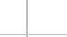
\includegraphics[max width=\textwidth]{2024_11_21_6438f6dbc3784fe6d1deg-08(4)}
 &  &  &  &  \\
\hline
 &  &  &  &  &  &  &  &  &  &  &  &  &  &  &  &  &  &  &  &  &  &  &  &  & 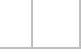
\includegraphics[max width=\textwidth]{2024_11_21_6438f6dbc3784fe6d1deg-08(1)}
 &  &  &  &  \\
\hline
\end{tabular}
\end{center}

Odpowiedź:

\section*{Zadanie 22. (2 pkt)}
Wierzchołek paraboli będącej wykresem funkcji kwadratowej \(f(x)=-3 x^{2}+12 x+c\) leży na prostej o równaniu \(y=x+1\). Oblicz wartość współczynnika \(c\).\\

\includegraphics[max width=\textwidth, center]{2024_11_21_6438f6dbc3784fe6d1deg-08(8)}

Odpowiedź: \(\qquad\)

\section*{Zadanie 23. (2 pkt)}
Zapisz wielomian \(W(x)=x^{3}+4 x^{2}-16 x-64 \mathrm{w}\) postaci iloczynowej. Uzasadnij, że dla każdej liczby rzeczywistej \(x \geq 4\) prawdziwa jest nierówność \(W(x) \geq 0\).

\begin{center}
\begin{tabular}{|c|c|c|c|c|c|c|c|c|c|c|c|c|c|c|c|c|c|c|c|c|c|c|c|c|c|c|c|c|c|}
\hline
 &  &  &  &  &  &  &  &  &  &  &  &  &  &  &  &  &  &  &  &  &  &  &  &  &  &  &  &  &  \\
\hline
 &  &  &  &  &  &  &  &  &  &  &  &  &  &  &  &  &  &  &  &  &  &  &  &  &  &  &  &  &  \\
\hline
 &  &  &  &  &  &  &  &  &  &  &  &  &  &  &  &  &  &  &  &  &  &  &  &  &  &  &  &  &  \\
\hline
 &  &  &  &  &  &  &  &  &  &  &  &  &  &  &  &  &  &  &  &  &  &  &  &  &  &  &  &  &  \\
\hline
 &  &  &  &  &  &  &  &  &  &  &  &  &  &  &  &  &  &  &  &  &  &  &  &  &  &  &  &  &  \\
\hline
 &  &  &  &  &  &  &  &  &  &  &  &  &  &  &  &  &  &  &  &  &  &  &  &  &  &  &  &  &  \\
\hline
 &  &  &  &  &  &  &  &  &  &  &  &  &  &  &  &  &  &  &  &  &  &  &  &  &  &  &  &  &  \\
\hline
 &  &  &  &  &  &  &  &  &  &  &  &  &  &  &  &  &  &  &  &  &  &  &  &  &  &  &  &  &  \\
\hline
 &  &  &  &  &  &  &  &  &  &  &  &  &  &  &  &  &  &  &  &  &  &  &  &  &  &  &  &  &  \\
\hline
 &  &  &  &  &  &  &  &  &  &  &  &  &  &  &  &  &  &  &  &  &  &  &  &  &  &  &  &  &  \\
\hline
 &  &  &  &  &  &  &  &  &  &  &  &  &  &  &  &  &  &  &  &  &  &  &  &  &  &  &  &  &  \\
\hline
 &  &  &  &  &  &  &  &  &  &  &  &  &  &  &  &  &  &  &  &  &  &  &  &  &  &  &  &  &  \\
\hline
 &  &  &  &  &  &  &  &  &  &  &  &  &  &  &  &  &  &  &  &  &  &  &  &  &  &  &  &  &  \\
\hline
 &  &  &  &  &  &  &  &  &  &  &  &  &  &  &  &  &  &  &  &  &  &  &  &  &  &  &  &  &  \\
\hline
 &  &  &  &  &  &  &  &  &  &  &  &  &  &  &  &  &  &  &  &  &  &  &  &  &  &  &  &  &  \\
\hline
 &  &  &  &  &  &  &  &  &  &  &  &  &  &  &  &  &  &  &  &  &  &  &  &  &  &  & 
\includegraphics[max width=\textwidth]{2024_11_21_6438f6dbc3784fe6d1deg-09}
 &  &  \\
\hline
 &  &  &  &  &  &  &  &  &  &  &  &  &  &  &  &  &  &  &  &  &  &  &  &  &  &  &  &  &  \\
\hline
 &  &  &  &  &  &  &  &  &  &  &  &  &  &  &  &  &  &  &  &  &  &  &  &  &  &  & 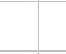
\includegraphics[max width=\textwidth]{2024_11_21_6438f6dbc3784fe6d1deg-09(1)}
 &  &  \\
\hline
 &  &  &  &  &  &  &  &  &  &  &  &  &  &  &  &  &  &  &  &  &  &  &  &  &  &  &  &  &  \\
\hline
\end{tabular}
\end{center}

Odpowiedź:

\section*{Zadanie 24. (2 pkt)}
Krótsza przekątna równoległoboku jest prostopadła do dwóch przeciwległych jego boków. Długość tej przekątnej jest o 3 cm większa od długości krótszego boku i o 3 cm mniejsza od długości dłuższego boku. Oblicz długość dłuższej przekątnej tego równoległoboku.

\begin{center}
\begin{tabular}{|c|c|c|c|c|c|c|c|c|c|c|c|c|c|c|c|c|c|c|c|c|c|c|c|c|c|c|c|c|c|c|}
\hline
 &  &  &  &  &  &  &  &  &  &  &  &  &  &  &  &  &  &  &  &  &  &  &  &  &  &  &  &  &  &  \\
\hline
 &  &  &  &  &  &  &  &  &  &  &  &  &  &  &  &  &  &  &  &  &  &  &  &  &  &  &  &  &  &  \\
\hline
 &  &  &  &  &  &  &  &  &  &  &  &  &  &  &  &  &  &  &  &  &  &  &  &  &  &  &  &  &  &  \\
\hline
 &  &  &  &  &  &  &  &  &  &  &  &  &  &  &  &  &  &  &  &  &  &  &  &  &  &  &  &  &  &  \\
\hline
 &  &  &  &  &  &  &  &  &  &  &  &  &  &  &  &  &  &  &  &  &  &  &  &  &  &  &  &  &  &  \\
\hline
 &  &  &  &  &  &  &  &  &  &  &  &  &  &  &  &  &  &  &  &  &  &  &  &  &  &  &  &  &  &  \\
\hline
 &  &  &  &  &  &  &  &  &  &  &  &  &  &  &  &  &  &  &  &  &  &  &  &  &  &  &  &  &  &  \\
\hline
 &  &  &  &  &  &  &  &  &  &  &  &  &  &  &  &  &  &  &  &  &  &  &  &  &  &  &  &  &  &  \\
\hline
 &  &  &  &  &  &  &  &  &  &  &  &  &  &  &  &  &  &  &  &  &  &  &  &  &  &  &  &  &  &  \\
\hline
 &  &  &  &  &  &  &  &  &  &  &  &  &  &  &  &  &  &  &  &  &  &  &  &  &  &  &  &  &  &  \\
\hline
 &  &  &  &  &  &  &  &  &  &  &  &  &  &  &  &  &  &  &  &  &  &  &  &  &  &  &  &  &  &  \\
\hline
 &  &  &  &  &  &  &  &  &  &  &  &  &  &  &  &  &  &  &  &  &  &  &  &  &  &  &  &  &  &  \\
\hline
 &  &  &  &  &  &  &  &  &  &  &  &  &  &  &  &  &  &  &  &  &  &  &  &  &  &  &  &  &  &  \\
\hline
 &  &  &  &  &  &  &  &  &  &  &  &  &  &  &  &  &  &  &  &  &  &  &  &  &  &  &  &  &  &  \\
\hline
 &  &  &  &  &  &  &  &  &  &  &  &  &  &  &  &  &  &  &  &  &  &  &  &  &  &  &  &  &  &  \\
\hline
 &  &  &  &  &  &  &  &  &  &  &  &  &  &  &  &  &  &  &  &  &  &  &  &  &  &  &  &  &  &  \\
\hline
 &  &  &  &  &  &  &  &  &  &  &  &  &  &  &  &  &  &  &  &  &  &  &  &  &  &  &  &  &  &  \\
\hline
 &  &  &  &  &  &  &  &  &  &  &  &  &  &  &  &  &  &  &  &  &  &  &  &  &  &  &  &  &  &  \\
\hline
\end{tabular}
\end{center}

Odpowiedź: \(\qquad\)\\
\(\qquad\)\\

\includegraphics[max width=\textwidth, center]{2024_11_21_6438f6dbc3784fe6d1deg-09(2)}

\section*{Zadanie 25. (2 pkt)}
Wewnątrz kwadratu \(A B C D\) wybrano takie punkty \(M\) i \(N\), że trójkąty \(A B M\) i \(B C N\) są równoboczne (zobacz rysunek). Udowodnij, że trójkąt \(D N M\) jest równoboczny.\\
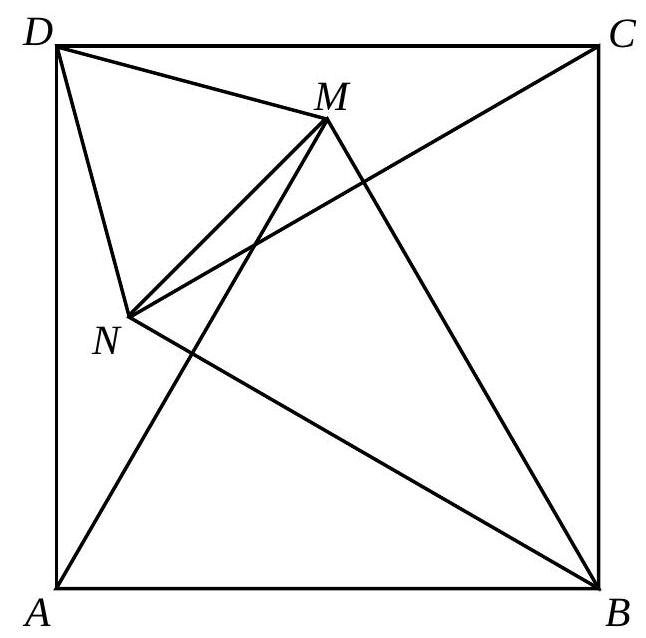
\includegraphics[max width=\textwidth, center]{2024_11_21_6438f6dbc3784fe6d1deg-10}\\

\includegraphics[max width=\textwidth, center]{2024_11_21_6438f6dbc3784fe6d1deg-10(1)}

Zadanie 26. (2 pkt)\\
Pierwszy odcinek łamanej ma długość 128 cm , a długość każdego następnego jej odcinka jest o 25\% mniejsza od długości poprzedniego. Najkrótszy odcinek tej łamanej ma długość \(40,5 \mathrm{~cm}\). Oblicz, z ilu odcinków składa się ta łamana.

\begin{center}
\begin{tabular}{|c|c|c|c|c|c|c|c|c|c|c|c|c|c|c|c|c|c|c|c|c|c|c|c|c|c|c|c|c|c|c|}
\hline
 &  &  &  &  &  &  &  &  &  &  &  &  &  &  &  &  &  &  &  &  &  &  &  &  &  &  &  &  &  &  \\
\hline
 &  &  &  &  &  &  &  &  &  &  &  &  &  &  &  &  &  &  &  &  &  &  &  &  &  &  &  &  &  &  \\
\hline
 &  &  &  &  &  &  &  &  &  &  &  &  &  &  &  &  &  &  &  &  &  &  &  &  &  &  &  &  &  &  \\
\hline
 &  &  &  &  &  &  &  &  &  &  &  &  &  &  &  &  &  &  &  &  &  &  &  &  &  &  &  &  &  &  \\
\hline
 &  &  &  &  &  &  &  &  &  &  &  &  &  &  &  &  &  &  &  &  &  &  &  &  &  &  &  &  &  &  \\
\hline
 &  &  &  &  &  &  &  &  &  &  &  &  &  &  &  &  &  &  &  &  &  &  &  &  &  &  &  &  &  &  \\
\hline
 &  &  &  &  &  &  &  &  &  &  &  &  &  &  &  &  &  &  &  &  &  &  &  &  &  &  &  &  &  &  \\
\hline
 &  &  &  &  &  &  &  &  &  &  &  &  &  &  &  &  &  &  &  &  &  &  &  &  &  &  &  &  &  &  \\
\hline
 &  &  &  &  &  &  &  &  &  &  &  &  &  &  &  &  &  &  &  &  &  &  &  &  &  &  &  &  &  &  \\
\hline
 &  &  &  &  &  &  &  &  &  &  &  &  &  &  &  &  &  &  &  &  &  &  &  &  &  &  &  &  &  &  \\
\hline
 &  &  &  &  &  &  &  &  &  &  &  &  &  &  &  &  &  &  &  &  &  &  &  &  &  &  &  &  &  &  \\
\hline
 &  &  &  &  &  &  &  &  &  &  &  &  &  &  &  &  &  &  &  &  &  &  &  &  &  &  &  &  &  &  \\
\hline
 &  &  &  &  &  &  &  &  &  &  &  &  &  &  &  &  &  &  &  &  &  &  &  &  &  &  &  &  &  &  \\
\hline
 &  &  &  &  &  &  &  &  &  &  &  &  &  &  &  &  &  &  &  &  &  &  &  &  &  &  &  &  &  &  \\
\hline
 &  &  &  &  &  &  &  &  &  &  &  &  &  &  &  &  &  &  &  &  &  &  &  &  &  &  &  &  &  &  \\
\hline
 &  &  &  &  &  &  &  &  &  &  &  &  &  &  &  &  &  &  &  &  &  &  &  &  &  &  &  &  &  &  \\
\hline
 &  &  &  &  &  &  &  &  &  &  &  &  &  &  &  &  &  &  &  &  &  &  &  &  &  &  &  &  &  &  \\
\hline
 &  &  &  &  &  &  &  &  &  &  &  &  &  &  &  &  &  &  &  &  &  &  &  &  &  &  &  &  &  &  \\
\hline
\end{tabular}
\end{center}

Odpowiedź: \(\qquad\)

\section*{Zadanie 27. (4 pkt)}
Ze zbioru \(\{2,3,4,5,6,7,8\}\) losujemy kolejno dwa razy po jednej liczbie bez zwracania. Oblicz prawdopodobieństwo zdarzenia, że iloczyn wylosowanych liczb będzie podzielny przez 6 lub przez 10.\\

\includegraphics[max width=\textwidth, center]{2024_11_21_6438f6dbc3784fe6d1deg-11}

Odpowiedź: \(\qquad\)

Zadanie 28. (5 pkt)\\
Wierzchołki trójkąta \(A B C\) mają współrzędne: \(A=(-4,7), B=(-2,-3)\) i \(C=(12,5)\). Punkt \(S\) jest środkiem boku \(B C\). Prosta \(A S\) przecina prostą do niej prostopadłą i przechodzącą przez punkt \(B\) w punkcie \(E\). Oblicz współzzędne punktu \(E\) i długość odcinka \(S E\).\\

\includegraphics[max width=\textwidth, center]{2024_11_21_6438f6dbc3784fe6d1deg-12}

Odpowiedź: \(\qquad\)

\section*{Zadanie 29. (4 pkt)}
Pole powierzchni całkowitej graniastosłupa prawidłowego sześciokątnego (zobacz rysunek) jest równe \(60 \sqrt{3}\). Krótsza przekątna tego graniastosłupa tworzy z płaszczyzną podstawy kąt \(\alpha\) taki, że \(\operatorname{tg} \alpha=2\). Oblicz długość krawędzi podstawy tego graniastosłupa.\\
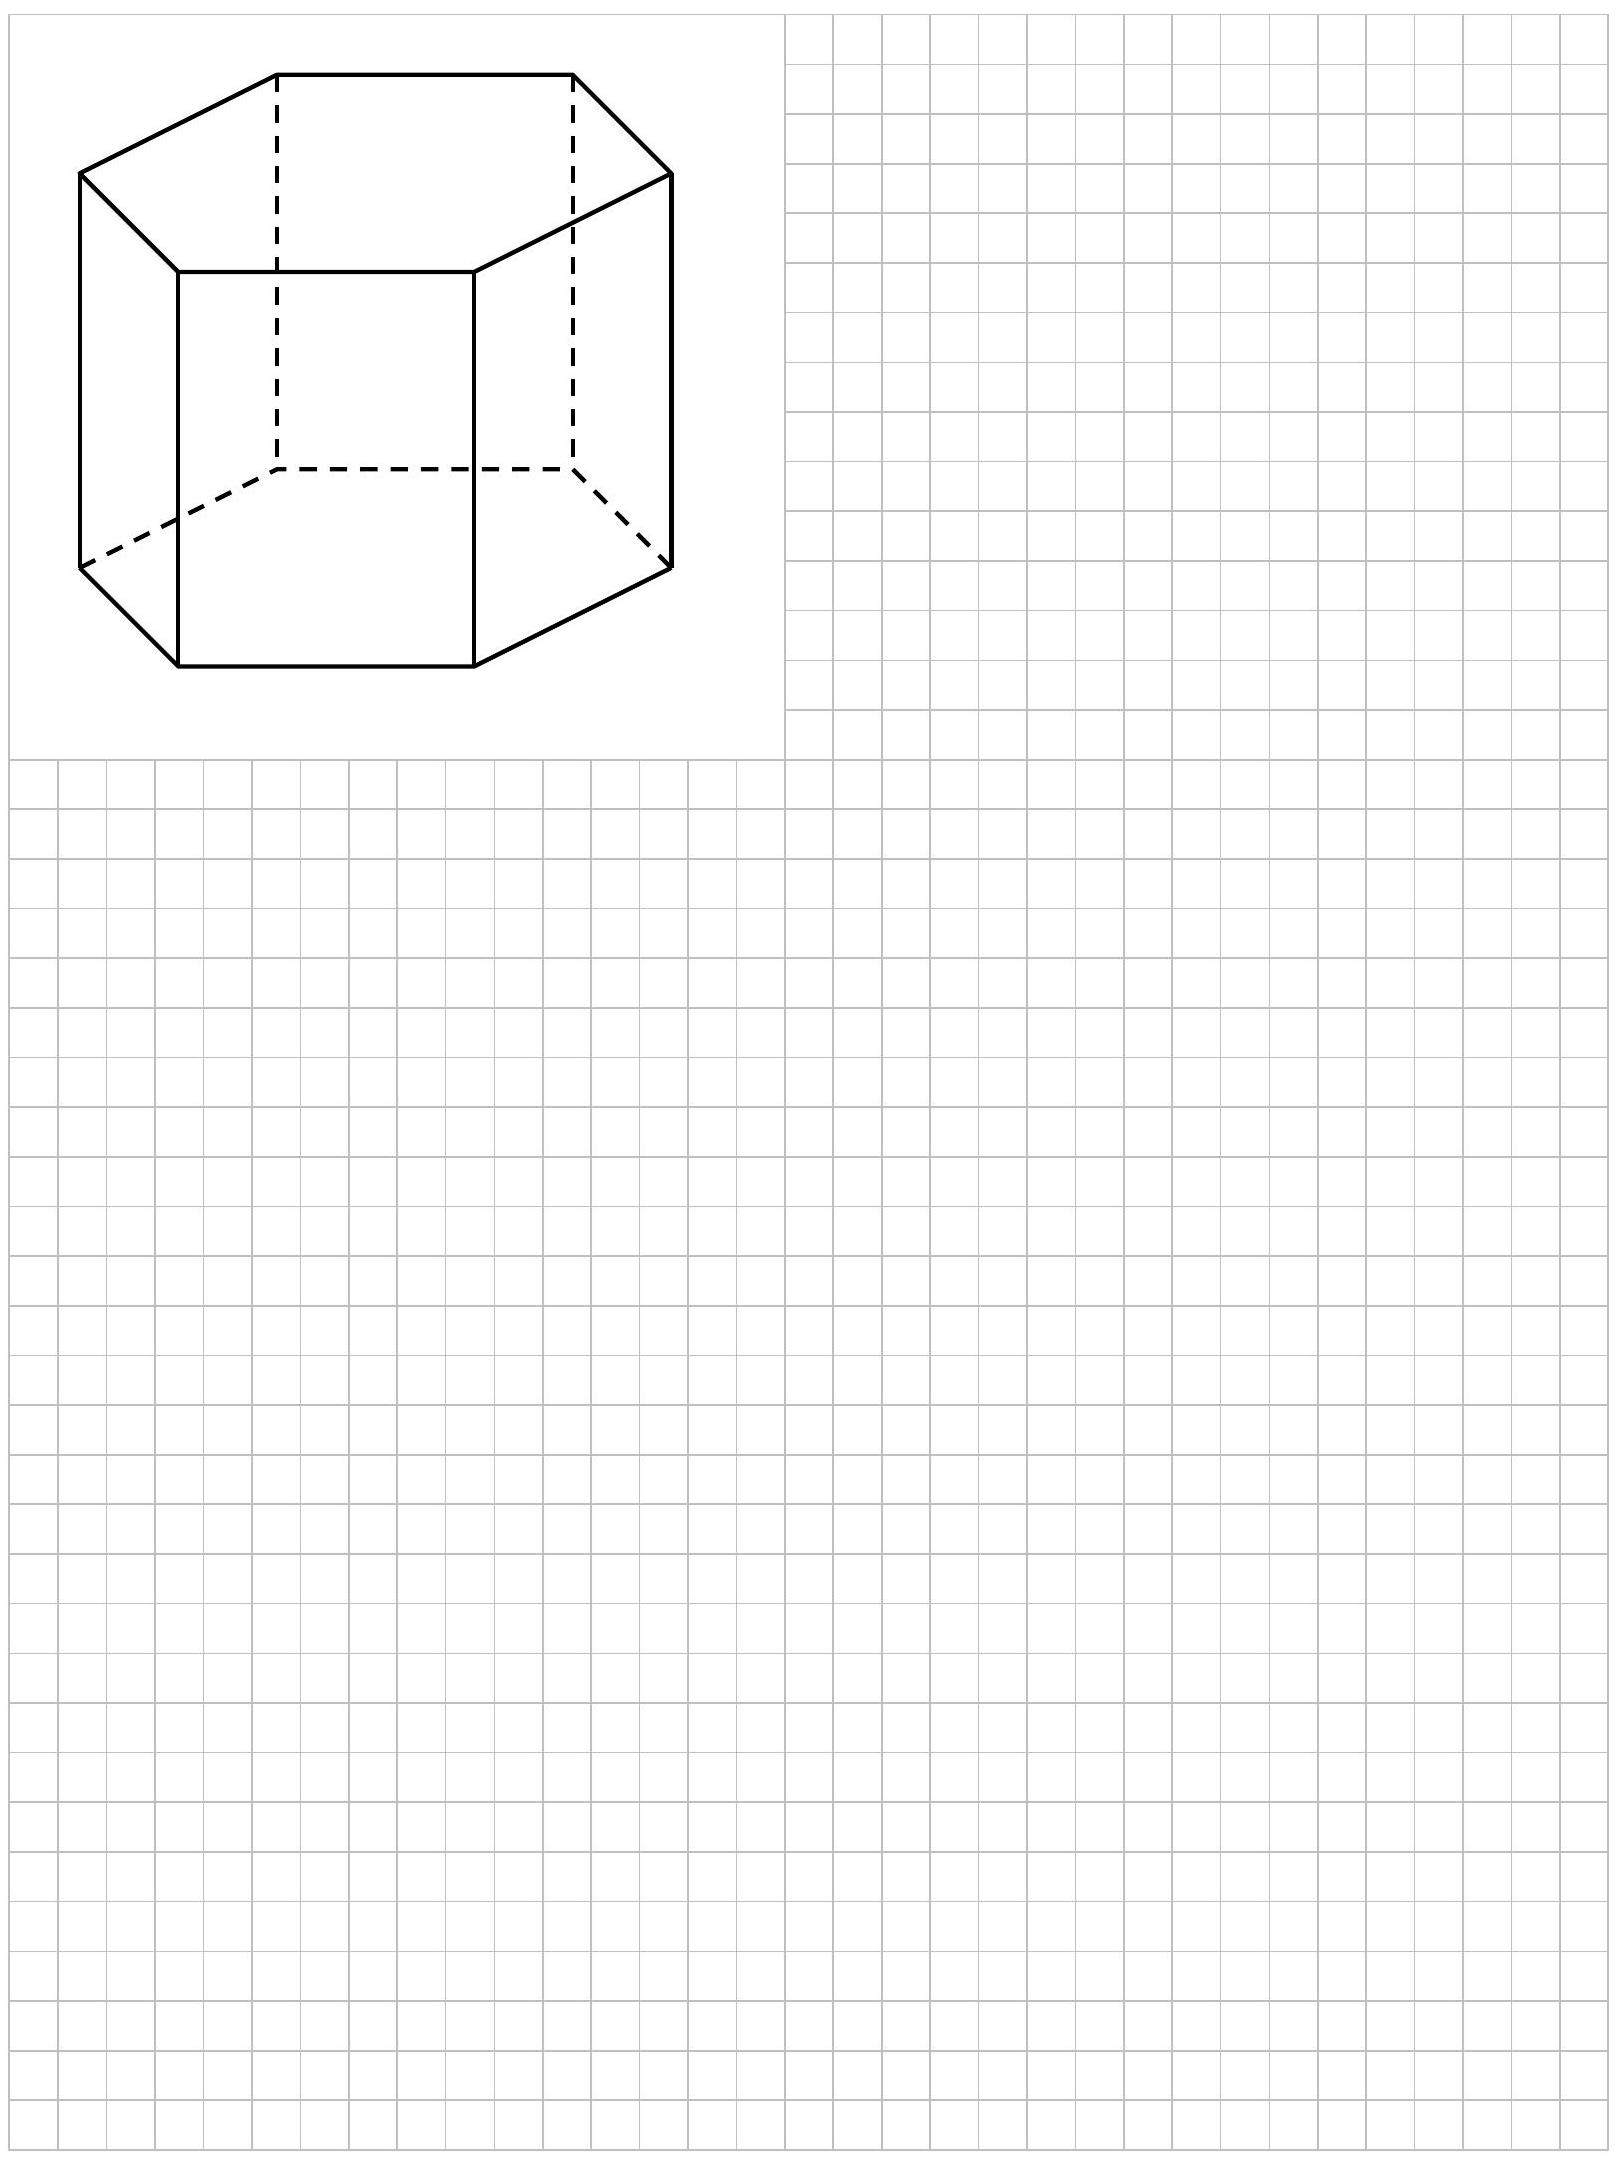
\includegraphics[max width=\textwidth, center]{2024_11_21_6438f6dbc3784fe6d1deg-13}

Odpowiedź: \(\qquad\)

\footnotetext{Odpowiedz
}Zadanie 30. (5 pkt)\\
Do zbiornika o pojemności \(800 \mathrm{~m}^{3}\) można doprowadzić wodę dwiema rurami. W ciągu jednej godziny pierwsza rura dostarcza do zbiornika o \(32 \mathrm{~m}^{3}\) wody więcej niż druga rura. Czas napełniania zbiornika tylko pierwszą rurą jest o 12 godzin i 30 minut krótszy od czasu napełniania tego zbiornika tylko drugą rurą. Oblicz, w ciągu ilu godzin pusty zbiornik zostanie napełniony, jeśli woda będzie doprowadzana przez obie rury jednocześnie.

\begin{center}
\begin{tabular}{|c|c|c|c|c|c|c|c|c|c|c|c|c|c|c|c|c|c|c|c|c|c|c|c|c|c|c|c|c|c|}
\hline
 &  &  &  &  &  &  &  &  &  &  &  &  &  &  &  &  &  &  &  &  &  &  &  &  &  &  &  &  &  \\
\hline
 &  &  &  &  &  &  &  &  &  &  &  &  &  &  &  &  &  &  &  &  &  &  &  &  &  &  &  &  &  \\
\hline
 &  &  &  &  &  &  &  &  &  &  &  &  &  &  &  &  &  &  &  &  &  &  &  &  &  &  &  &  &  \\
\hline
 &  &  &  &  &  &  &  &  &  &  &  &  &  &  &  &  &  &  &  &  &  &  &  &  &  &  &  &  &  \\
\hline
 &  &  &  &  &  &  &  &  &  &  &  &  &  &  &  &  &  &  &  &  &  &  &  &  &  &  &  &  &  \\
\hline
 &  &  &  &  &  &  &  &  &  &  &  &  &  &  &  &  &  &  &  &  &  &  &  &  &  &  &  &  &  \\
\hline
 &  &  &  &  &  &  &  &  &  &  &  &  &  &  &  &  &  &  &  &  &  &  &  &  &  &  &  &  &  \\
\hline
 &  &  &  &  &  &  &  &  &  &  &  &  &  &  &  &  &  &  &  &  &  &  &  &  &  &  &  &  &  \\
\hline
 &  &  &  &  &  &  &  &  &  &  &  &  &  &  &  &  &  &  &  &  &  &  &  &  &  &  &  &  &  \\
\hline
 &  &  &  &  &  &  &  &  &  &  &  &  &  &  &  &  &  &  &  &  &  &  &  &  &  &  &  &  &  \\
\hline
 &  &  &  &  &  &  &  &  &  &  &  &  &  &  &  &  &  &  &  &  &  &  &  &  &  &  &  &  &  \\
\hline
 &  &  &  &  &  &  &  &  &  &  &  &  &  &  &  &  &  &  &  &  &  &  &  &  &  &  &  &  &  \\
\hline
 &  &  &  &  &  &  &  &  &  &  &  &  &  &  &  &  &  &  &  &  &  &  &  &  &  &  &  &  &  \\
\hline
 &  &  &  &  &  &  &  &  &  &  &  &  &  &  &  &  &  &  &  &  &  &  &  &  &  &  &  &  &  \\
\hline
 &  &  &  &  &  &  &  &  &  &  &  &  &  &  &  &  &  &  &  &  &  &  &  &  &  &  &  &  &  \\
\hline
 &  &  &  &  &  &  &  &  &  &  &  &  &  &  &  &  &  &  &  &  &  &  &  &  &  &  &  &  &  \\
\hline
 &  &  &  &  &  &  &  &  &  &  &  &  &  &  &  &  &  &  &  &  &  &  &  &  &  &  &  &  &  \\
\hline
 &  &  &  &  &  &  &  &  &  &  &  &  &  &  &  &  &  &  &  &  &  &  &  &  &  &  &  &  &  \\
\hline
 &  &  &  &  &  &  &  &  &  &  &  &  &  &  &  &  &  &  &  &  &  &  &  &  &  &  &  &  &  \\
\hline
 &  &  &  &  &  &  &  &  &  &  &  &  &  &  &  &  &  &  &  &  &  &  &  &  &  &  &  &  &  \\
\hline
 &  &  &  &  &  &  &  &  &  &  &  &  &  &  &  &  &  &  &  &  &  &  &  &  &  &  &  &  &  \\
\hline
 &  &  &  &  &  &  &  &  &  &  &  &  &  &  &  &  &  &  &  &  &  &  &  &  &  &  &  &  &  \\
\hline
 &  &  &  &  &  &  &  &  &  &  &  &  &  &  &  &  &  &  &  &  &  &  &  &  &  &  &  &  &  \\
\hline
 &  &  &  &  &  &  &  &  &  &  &  &  &  &  &  &  &  &  &  &  &  &  &  &  &  &  &  &  &  \\
\hline
 &  &  &  &  &  &  &  &  &  &  &  &  &  &  &  &  &  &  &  &  &  &  &  &  &  &  &  &  &  \\
\hline
 &  &  &  &  &  &  &  &  &  &  &  &  &  &  &  &  &  &  &  &  &  &  &  &  &  &  &  &  &  \\
\hline
 &  &  &  &  &  &  &  &  &  &  &  &  &  &  &  &  &  &  &  &  &  &  &  &  &  &  &  &  &  \\
\hline
 &  &  &  &  &  &  &  &  &  &  &  &  &  &  &  &  &  &  &  &  &  &  &  &  &  &  &  &  &  \\
\hline
 &  &  &  &  &  &  &  &  &  &  &  &  &  &  &  &  &  &  &  &  &  &  &  &  &  &  &  &  &  \\
\hline
 &  &  &  &  &  &  &  &  &  &  &  &  &  &  &  &  &  &  &  &  &  &  &  &  &  &  &  &  &  \\
\hline
 &  &  &  &  &  &  &  &  &  &  &  &  &  &  &  &  &  &  &  &  &  &  &  &  &  &  &  &  &  \\
\hline
 &  &  &  &  &  &  &  &  &  &  &  &  &  &  &  &  &  &  &  &  &  &  &  &  &  &  &  &  &  \\
\hline
 &  &  &  &  &  &  &  &  &  &  &  &  &  &  &  &  &  &  &  &  &  &  &  &  &  &  &  &  &  \\
\hline
 &  &  &  &  &  &  &  &  &  &  &  &  &  &  &  &  &  &  &  &  &  &  &  &  &  &  &  &  &  \\
\hline
 &  &  &  &  &  &  &  &  &  &  &  &  &  &  &  &  &  &  &  &  &  &  &  &  &  &  &  &  &  \\
\hline
 &  &  &  &  &  &  &  &  &  &  &  &  &  &  &  &  &  &  &  &  &  &  &  &  &  &  &  &  &  \\
\hline
 &  &  &  &  &  &  &  &  &  &  &  &  &  &  &  &  &  &  &  &  &  &  &  &  &  &  &  &  &  \\
\hline
 &  &  &  &  &  &  &  &  &  &  &  &  &  &  &  &  &  &  &  &  &  &  &  &  &  &  &  &  &  \\
\hline
 &  &  &  &  &  &  &  &  &  &  &  &  &  &  &  &  &  &  &  &  &  &  &  &  &  &  &  &  &  \\
\hline
 &  &  &  &  &  &  &  &  &  &  &  &  &  &  &  &  &  &  &  &  &  &  &  &  &  &  &  &  &  \\
\hline
 &  &  &  &  &  &  &  &  &  &  &  &  &  &  &  &  &  &  &  &  &  &  &  &  &  &  &  &  &  \\
\hline
 &  &  &  &  &  &  &  &  &  &  &  &  &  &  &  &  &  &  &  &  &  &  &  &  &  &  &  &  &  \\
\hline
\end{tabular}
\end{center}

Odpowiedź: \(\qquad\)

\section*{BRUDNOPIS}
\section*{KARTA ODPOWIEDZI}
\section*{WYPEŁNIA ZDAJĄCY}
PESEL\\
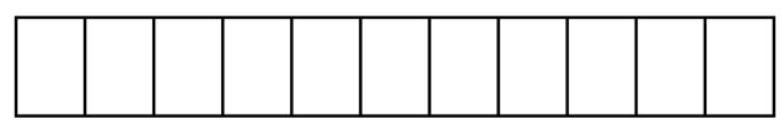
\includegraphics[max width=\textwidth, center]{2024_11_21_6438f6dbc3784fe6d1deg-16(1)}

\begin{center}
\begin{tabular}{|c|c|c|c|c|}
\hline
 & \multicolumn{4}{|c|}{Odpowiedzi} \\
\hline
1 & ( & B & C &  \\
\hline
2 & ( & B & C & D \\
\hline
3 & * & B & C & D \\
\hline
4 & * & B & C & ■ \\
\hline
5 & ( & B & C & ■ \\
\hline
6 & ( & B & C & D \\
\hline
7 & ( & B & C & D \\
\hline
8 & ( & B & C & D \\
\hline
9 & ( & B & C & D \\
\hline
10 & ( & B & C & ■ \\
\hline
11 & ( & B & C & D \\
\hline
12 & ( & B & C & D \\
\hline
13 & ( & B & C & D \\
\hline
14 & ( & B & C & D \\
\hline
15 &  & B & C & 回 \\
\hline
16 & ( & B & C & D \\
\hline
17 &  & B & C & D \\
\hline
18 & ( & B & C & D \\
\hline
19 & ( & B & C & D \\
\hline
20 &  & B & C & D \\
\hline
\end{tabular}
\end{center}

WYPEŁNIA EGZAMINATOR

\begin{center}
\begin{tabular}{|c|c|c|c|c|c|c|}
\hline
\multirow{2}{*}{\begin{tabular}{c}
Nr \\
zadania \\
\end{tabular}} & \multicolumn{6}{|c|}{Punkty} \\
\hline
 & \(\square\) & \(\square\) & \(\square\) &  &  &  \\
\hline
22 & \(\square\) & \(\square\) & \(\square\) &  &  &  \\
\hline
23 & \(\square\) & \(\square\) & \(\square\) &  &  &  \\
\hline
24 & \(\square\) & \(\square\) & \(\square\) &  &  &  \\
\hline
25 & \(\square\) & \(\square\) & \(\square\) &  &  &  \\
\hline
26 & \(\square\) & \(\square\) & \(\square\) & \(\square\) &  &  \\
\hline
27 & \(\square\) & \(\square\) & \(\square\) & \(\square\) & \(\square\) &  \\
\hline
28 & \(\square\) & \(\square\) & \(\square\) & \(\square\) & \(\square\) & \(\square\) \\
\hline
29 & \(\square\) & \(\square\) & \(\square\) & \(\square\) & \(\square\) &  \\
\hline
30 & \(\square\) & \(\square\) & \(\square\) & \(\square\) & \(\square\) & \(\square\) \\
\hline
\end{tabular}
\end{center}

\begin{center}
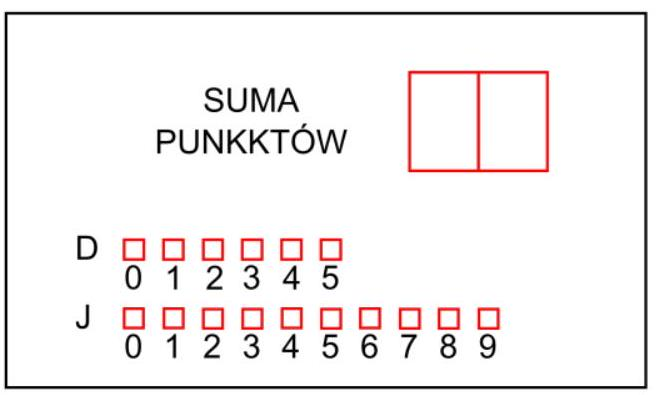
\includegraphics[max width=\textwidth]{2024_11_21_6438f6dbc3784fe6d1deg-16}
\end{center}


\end{document}